%!TEX TS-program = xelatex
\documentclass[]{friggeri-cv}
\usepackage{afterpage}
\usepackage{hyperref}
\usepackage{color}
\usepackage{xcolor}
\hypersetup{
    pdftitle={},
    pdfauthor={},
    pdfsubject={},
    pdfkeywords={},
    colorlinks=false,       % no lik border color
   allbordercolors=white    % white border color for all
}
\RequirePackage{xcolor}
\definecolor{pblue}{HTML}{0395DE}

\usepackage{enumitem}

\begin{document}
\header{Victor M.}{Mendiola-Lau}{Computer Scientist, Researcher and Software Engineer}
      
% Fake text to add separator      
\fcolorbox{white}{gray}{\parbox{\dimexpr\textwidth-2\fboxsep-2\fboxrule}{%
.....
}}

% In the aside, each new line forces a line break
\begin{aside}
  \section{Address}
    Jaén, Jaén, Spain
    ~
    ~
    ~
  \section{Telephone}
    (+34) 621 06 15 01
    ~
    ~
    ~
  \section{Mail}
    \href{mailto:ryuzakyl@gmail.com}{\textbf{ryuzakyl@}gmail.com}
	~
	~    
    ~
  \section{Web profiles}
    \href{https://github.com/ryuzakyl}{{\scriptsize github.com/ryuzakyl}}
    \href{https://independent.academia.edu/VictorMendiolaLau}{{\scriptsize academia.edu/VictorMendiolaLau}}
    \href{https://www.linkedin.com/in/VictorMendiolaLau}{{\scriptsize linkedin.com/in/VictorMendiolaLau}}
	\href{https://www.researchgate.net/profile/Victor_Mendiola-Lau}{{\scriptsize researchgate.net/Victor\char`_Mendiola-Lau}}
    ~
    ~
    ~
  \section{Personal Skills}
    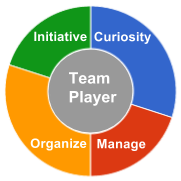
\includegraphics[scale=0.62]{img/personal.png}
    ~
%    ~
%  \section{Programming}
%    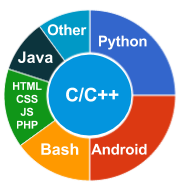
\includegraphics[scale=0.62]{img/programming.png}
%    ~
\end{aside}

\section{Software Engineering}
\begin{entrylist}
  \entry
    {11/19 - Now}
    {Full Stack Web Developer}
    % {Iversoft - Digital consultancy & technology partner. (https://www.iversoft.ca/)}
    {}
    {Construction of an organization's website. Technologies: Wordpress, PHP, HTML, CSS3, JavaScript, MySQL, etc.\\} 

  \entry
    {09/18 - 09/19}
    {Software Engineer}
    {Kitsune Technologies, Tennessee, USA}   
    {Wide range of responsibilities including Data Analysis, Computer Vision, Web development, services implementation, etc.\\}

  \entry
    {09/17 - 11/18}
    {Full Stack Web Developer}
    % {HRSG - Human Resource Systems Group Ltd. (https://www.hrsg.ca/)}
    {}
    {Web-based applications as solutions to workforce management. Technologies: PHP, HTML, CSS3, JavaScript, jQuery, MySQL, etc.\\} 

  \entry
    {12/17 - 02/18}
    {Python/Django Backend Developer}
    {SBY Technologies, Florida, USA}   
    {Developed a REST API from the ground up with JWT Authentication, automatic reports generation (.pdf, .csv), etc. Also worked as a DevOps Engineer and Linux System Administrator.\\}    

  \entry
    {02/16 - 03/16}
    {Ruby/Rails Backend Developer}
    {Ksabes, Havana, Cuba}
    {Completely engineered and developed an API relying on Json Web Token (JWT) for authentication.\\}
  
  \entry
    {09/14 - 01/15}
    {Ruby Developer}
    {IRStrat, México D.F., México}
    {Completely engineered and developed a multi-threaded and concurrent service for consuming real time stock market data.\\}
    
  \entry
    {09/13 - 09/17}
    {Software Engineer}
    {CENATAV, Havana, Cuba}
    {.NET/C++ Software Engineer (Desktop, SDKs, etc.). Efficient algorithm design and implementation in C/C++/C\#. Applications integration with C/C++ libraries via PInvoke.\\}
\end{entrylist}

\section{Research \& Teaching}
\begin{entrylist}
  \entry
    {09/18 - 12/18}
    {Visiting Researcher}
    {University of Seville, Spain}
    {Researcher in topics like Machine Learning and Data Analysis.\\}

  \entry
    {10/17 - 09/18}
    {Instructor Professor}
    {University of Havana, Cuba}
    {Math instructor of topics such as Set theory, Functions, Algebra, Calculus, Numerical math and Ordinary Differential Equations.\\}

  \entry
    {09/13 - 09/17}
    {Researcher}
    {CENATAV, Havana, Cuba}
    {Design and development of Pattern Recognition Systems. Junior researcher and PhD. student. Interest on topics like Machine Learning, Data Analysis, Data Representation and Computer Vision. Technologies: Python, Numpy, SciPy, Matplotlib, scikit-learn, etc.\\}
\end{entrylist}

\begin{entrylist}
  \entry
    {06/12 - 07/12}
    {Research internship}
    {CENATAV, Havana, Cuba}
    {Design and implementation of an iris encoding method based on Functional Data Analysis (FDA).\\}
    
  \entry
    {09/10 - 06/13}
    {Assistant Instructor}
    {University of Havana, Cuba}
    {Instructor of Programming and Algorithms for Mathematics students in the Faculty of Mathematics and Computer Science (MATCOM).\\}
\end{entrylist}

\section{Other responsibilities}
\begin{entrylist}
  \entry
    {11/18 - 10/19}
    {Consultant}
    {PNWA, Seattle, USA}
    {Member of the Pacific NorthWest Advisors (PNWA) consulting group conducting informatics and market research inside Cuba, also providing unique insights to Pacific Northwest firms.}
\end{entrylist}

\section{Education/Academic background}
\begin{entrylist}
  \entry
    {2019 - }
    {Master's Degree in Cyber Security}
    {University of Jaén, Spain}
    {
    	Main subjects: Secure Cloud Applications, Network Security, Intrusion Detection, Reverse Engineering, Malware Analysis, Advanced Cryptography.\\
%    	\emph{Title of the Thesis: "A Handoff Algorithm based on Link Quality Prediction for Mass Transit Wireless Mesh Networks".}\\
%    	\emph{Relators: Prof. Enzo Mingozzi, Ing. Carlo Vallati, Prof. Luciano Lenzini.}\\
    }

  \entry
    {2008 - 2013}
    {B.Sc. in Computer Science}
    {University of Havana, Cuba}
    {B.Sc. in Computer Science (5.13 of 5.0).\\ Main subjects: Programming, Algorithms and Data Structures, Computational Complexity Theory, Matematics, Operational Research, Numerical Matematics and Artificial Intelligence.\\
    \emph{Title of the Thesis: "Iris Recognition using Functional Data Analysis (FDA)".}}

%  \entry
%    {2004 - 2007}
%    {Bachelor Diploma}
%    {IPVCE Vladimir Ilich Lenin, Havana, Cuba}
%    {Bachelor diploma with focus on these subjects: Matematics and Computer Science.}
\end{entrylist}

\section{Languages}
\begin{entrylist}
  \entry
    {\textbf{Spanish}}
    {}
    {}
    {Native tongue}      

  \entry
    {\textbf{English}}
    {}
    {}
    {
    	\textbf{Proficient user}: IELTS score 7.0 overall (corresponding to \textbf{C1} in CEFR). 
    	Graduated \textbf{\emph{summa cum laude}} at \emph{Abraham Lincoln} Languages School.\\
    }

  \entry
    {\textbf{French}}
    {}
    {}
    {Diplôme d'études en langue française (\textbf{DELF B2}) à l'Alliance française.}
\end{entrylist}

\section{Certifications \& Training courses}
\begin{entrylist}
  \entry
    {2014}
    {(Postgraduate) Methodologies of Scientific Research}
    {CENATAV, IDICT}
    {\emph{Demistify research and research methods. Outline of the fundamentals of doing research.}}
\end{entrylist}

\begin{entrylist}    
  \entry
    {2013}
    {(Tutorial) Fundamentals of Iris Recognition}
    {CIARP 2013 Congress}
    {\emph{Tutorial presented by Professor Tieniu Tan on the roadmap of Iris Recognition.}}

  \entry
    {}
    {(Tutorial) Big Data Analytics}
    {CIARP 2013 Congress}
    {\emph{Mining Uncertain and Probabilistic Data for Big Data Analytics by Professor Jian Pei.}}
    
  \entry
    {}
    {(Undergraduate) \LaTeX}
    {University of Havana}
    {\emph{Introduction to the document description language built on top of \TeX.}}
\end{entrylist}
       
\begin{entrylist}
  \entry
    {2012}
    {(Postgraduate) Advanced Data Structures}
    {University of Havana}
    {\emph{Introduction concepts such as Amortized Analysis, Fibonacci Heaps, Splay Trees, etc.}}      

  \entry
    {}
    {(Undergraduate) Business Intelligence}
    {University of Havana}
    {\emph{Introduction to the core concepts of modern Business Intelligence processes.}}

  \entry
    {}
    {(Undergraduate) Introduction to Cryptography}
    {University of Havana}
    {\emph{Introduction to the fundamentals of modern Cryptography.}}
\end{entrylist}

\begin{entrylist}
  \entry
    {2011}
    {(Undergraduate) Introduction to Computer Vision}
    {University of Havana}
    {\emph{Foundations of Computer Vision with OpenCV.}}      

  \entry
    {}
    {(Undergraduate) Introduction to Computer Graphics}
    {University of Havana}
    {\emph{Foundations of Computer Graphics.}}
\end{entrylist}

\section{Technologies}
\begin{entrylist}
  \entry
    {\textbf{Languages}}
    {}
    {}
    {\textbf{C\#} (+9 years), \textbf{Python} (+7 years), \textbf{C/C++} (+5 years), \textbf{Ruby} (+2 years), \textbf{PHP} (+2 años). Other languages include \textbf{Go} and \textbf{Java}.}

  \entry
    {\textbf{IDEs\&Editors}}
    {}
    {}
    {\textbf{Visual Studio}, \textbf{VS Code} and \textbf{JetBrains IDEs}.}
\end{entrylist}

\begin{entrylist}
  \entry
    {\textbf{ML \& DA}}
    {}
    {}
    {The Python stack for Machine Learning and Data Analysis: \textbf{Numpy}, \textbf{SciPy}, \textbf{Pandas}, \textbf{scikit-learn} and \textbf{Matplotlib}. Also the \textbf{MATLAB} programming language and environment.}

  \entry
    {\textbf{Web}}
    {}
    {}
    {\textbf{HTML}, \textbf{CSS3}, \textbf{JavaScript}, \textbf{Vue.js}, \textbf{jQuery}, \textbf{PHP}, \textbf{Django}, \textbf{Django Rest Framework}, \textbf{ASP.NET MVC/Core} and \textbf{Ruby on Rails}.}

  \entry
    {\textbf{Cloud}}
    {}
    {}
    {\textbf{AWS} and \textbf{Google Cloud Platform}.}

  \entry
    {\textbf{Desktop}}
    {}
    {}
    {\textbf{.NET}, \textbf{.NET Core} and \textbf{Qt}.}

  \entry
    {\textbf{DVCS}}
    {}
    {}
    {\textbf{Git} (+5 years) (\textbf{GitHub}, \textbf{GitLab} and \textbf{Bitbucket}).}
    
  \entry
    {\textbf{DBMS}}
    {}
    {}
    {\textbf{PostgreSQL}, \textbf{Microsoft SQL Server}, \textbf{MySQL} and \textbf{SQLite}.}
    
  \entry
    {\textbf{CV}}
    {}
    {}
    {\textbf{OpenCV}, \textbf{EmguCV} and \textbf{OpenCV-Python bindings}.}      
    
  \entry
    {\textbf{OS}}
    {}
    {}
    {\textbf{GNU/Linux} (+4 years) (\textbf{Ubuntu}, \textbf{Linux Mint}) y \textbf{Microsoft Windows} (+15 years).}
\end{entrylist}
\\
\section{Other Accomplishments}
\begin{itemize}[noitemsep, nolistsep]

	\item Achieved a GPA of 5.13 over a scale of 5.0\footnote{The extra points were the result of outstanding academic achievements.}.\\

	\item ACM-ICPC Cuban Finals contestant (2011 and 2013 editions)\footnote{Competed for a spot in ACM-ICPC Caribbean Finals contest.}.\\

	\item Winner of the $1^{st}$ prize at the 2010-2011 Scientific Journal of the Faculty of Mathematics and Computer Science.\\
	
	\item I have made some contributions to the Wikipedia article entitled ``\emph{Computational complexity theory}".\\
		
	\item Winner of the silver medal in Mathematics of the $12^{ve}$ grade in Havana.\\
	
	% \item From 2004 until 2007 was selected as part of advanced groups in Mathematics.\\	
	
	% \item Best candidate\footnote{Highest grade.} of the \emph{Plaza de la Revolución} locality at the IPVCE Vladimir Ilich Lenin admission tests in 2003-2004.\\	
	
	% \item Valedictorian from my elementary school in 2001.\\	
	
\end{itemize}

\end{document}
